\chapter{\IfLanguageName{dutch}{Stand van zaken}{State of the art}}
\label{ch:stand-van-zaken}

% Tip: Begin elk hoofdstuk met een paragraaf inleiding die beschrijft hoe
% dit hoofdstuk past binnen het geheel van de bachelorproef. Geef in het
% bijzonder aan wat de link is met het vorige en volgende hoofdstuk.

% Pas na deze inleidende paragraaf komt de eerste sectiehoofding.

Dit onderzoek heeft als doel om, uit drie kandidaten, één end-to-end testing framework aan te duiden dat het meest geschikt is voor de use case van Colruyt Group, zoals beschreven in het voorgaande hoofdstuk. Deze drie kandidaat-frameworks zijn de volgende:

\begin{enumerate}
    \item Protractor
    \item Cypress
    \item UFT
\end{enumerate}

In dit hoofdstuk worden eerst de principes van een robuuste testarchitectuur besproken. Dit om de nodige context te geven voor de drie kandidaat-frameworks, die daarna besproken worden. Ten slotte worden drie zogeheten ``Behavior Driven Development'' (BDD) frameworks onder de loep genomen. Deze frameworks zijn een extra laag bovenop een testing framework en maken het mogelijk acceptatietesten in quasi natuurlijke taal te schrijven, wat de implementatie versnelt (\cite{Diepenbeck2014}).

\section{Testing Architectuur}

De consensus is dat grofweg 50\% van de middelen van een softwareproject besteed worden aan de testfase (~\cite{Kasurinen2010,Tsai2001,Dadwal2018}). Er is met andere woorden een sterk (financieel) motief om dit aandeel te verkleinen middels test automatisatie.

Wie het implementeren van test automatisatie overweegt, dient er zich bewust van te zijn dat de kosten daarvan hoger zijn tijdens de eerste release van het test automatisatiesysteem \autocite{Fewster2001} \autocite{Kumar2016}. Dit is althans het geval wanneer men een minimale onderhoudskost nastreeft. In dit geval kunnen de kosten geassocieerd met test automatisatie op \emph{lange} termijn echter gereduceerd worden tot minder dan de helft van de kost om het testen 100\% manueel uit te voeren \autocite{Kumar2016}.

Een bijkomend voordeel is dat de vrijgekomen tijd bij het testing team gebruikt kan worden voor de meest complexe en veeleisende test cases (\cite{Barrett2013}).

Eerder onderzoek door Persson en Yilmaztürk wees uit dat de onderhoudbaarheid van een test automatisatiesysteem ondergeschikt maken aan het gemak van implementatie een groter risico op falen met zich meebrengt \autocite{Persson2004}. Een weloverwogen testarchitectuur is met andere woorden onontbeerlijk voor het slagen van een test automatisatiesysteem. Sterker nog: het ontwikkelingsproces van een test automatisatiesysteem zou vrijwel analoog moeten zijn aan dat van de eigenlijke software \autocite{Pettichord1996}.

\subsection{Multitierarchitectuur}

Bij het ontwikkelen van software volgens de Agile filosofie is het noodzakelijk (geautomatiseerde) test cases continu te herwerken om ze representatief te houden \autocite{Day2014}. Een test automatisatiesysteem dat gebaseerd is op een multitierarchitectuur (ook: n-tier architectuur) kan de onderhoudskosten desondanks relatief laag houden.

Concreet zal een multitierarchitectuur de verschillende soorten functionaliteit uit elkaar halen en los van elkaar testen. Idealiter zou elk van de lagen van de software vervangen moeten kunnen worden door één van de test automatisatielagen zonder hierdoor fouten of onverwacht gedrag te introduceren \autocite{Anandan}. Day stelt zelf 4 standaardtiers voor:

\begin{enumerate}
    \item ``Presentation'': de grafische interface en gebruikerservaring, die vaak middels \emph{smoke style testing}\footnote{\textbf{Smoke testing} focust zich op een handvol eenvoudige testen om de meest voor de hand liggende scenario's te valideren en zware fouten er uit te halen \autocite{Klostermann2019}.} gevalideerd wordt
    \item ``Business'': domeinlogica, die in de meeste gevallen het grootste aandeel te testen functionaliteit vertegenwoordigd
    \item ``Data'': opslag en ophalen van gegevens
    \item ``Web Services''
\end{enumerate}

De tiers kunnen evengoed georganizeerd worden in een \emph{front-end} (de grafische gebruikersomgeving) en een \emph{back-end} (logica, data en services) view, zoals ook Day doet in zijn case study.

\subsection{End-to-End Testing}

Een mulitierarchitectuur laat toe softwaremodules in afzondering te valideren, wat het mogelijk maakt fouten snel en met grote nauwkeurigheid te identificeren. Om te kunnen stellen dat een gegeven softwareproduct aan de vooropgestelde kwaliteitseisen voldoet, moet dat product echter ook als een geheel én in zijn gebruikscontext gevalideerd worden. Dit gebeurt hoofdzakelijk op twee manieren \autocite{Tsai2001}:

\begin{enumerate}
    \item ``Integratietesting'': test meerdere modules als groep (subsysteem) 
    \item ``End-to-End (E2E) (integratie)testing'': testen van de functionaliteit van een applicatie vanuit een \textbf{gebruikersstandpunt}, vindt normaliter plaats na de integratietesting
\end{enumerate}

\subsubsection{Thin Threads}

Tsai et al. stellen in hun paper van 2001 een aanpak voor het ontwerpen van E2E testingsystemen voor die zich focust op zogeheten ``\textbf{thin threads}''. Elke thin-thread vertegenwoordigd één gebruikersscenario, heeft een aantal voorwaarden (``condities'') en kent eventueel input- en/of outputgegevens. \textbf{Condities} kunnen te maken hebben met gegevens (verplichtheid van en vereisten gesteld aan de data), communicatie (time-outs en recovery mechanismen, security), de volgorde van operaties (coördinatie, updates) of eventuele andere factoren.

Zowel thin-threads als hun condities hebben onderlinge relaties en kunnen in een boomstructuur georganiseerd worden.

\begin{figure}[h!]
    \centering
    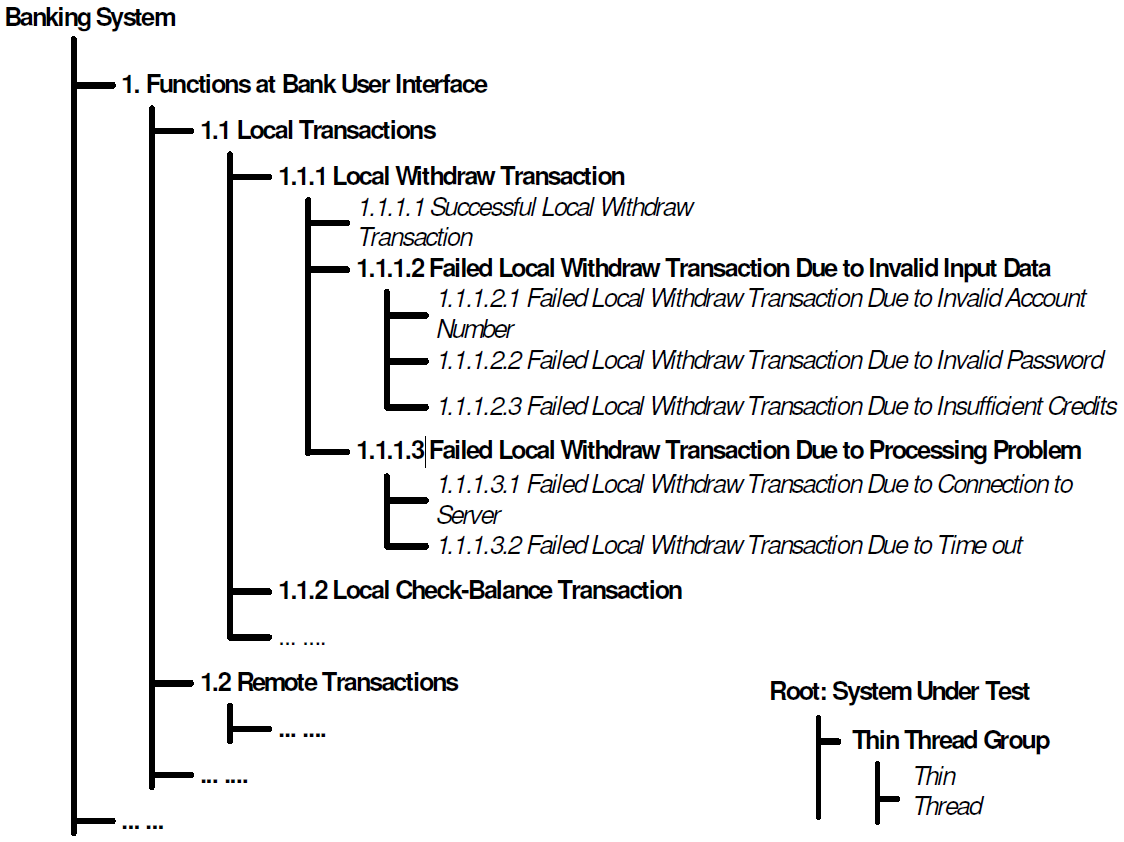
\includegraphics[scale=0.45]{img/Tsai2001ThinThreadTree.png}
    \caption{Een hypothetische thin-thread boom voor een bankiersapplicatie \autocite{Tsai2001}}
    \label{fig:tsaithinthreadtree}
\end{figure}

De relaties tussen thin-threads onderling worden bepaald door hoe hun uitvoeringspaden zich tot elkaar verhouden:

\begin{enumerate}
    \item ``Deel-geheel'': het pad van één thin-thread is deel van dat van een andere thin-thread
    \item ``Identiek'': de paden zijn identiek; ze delen condities of andere eigenschappen
    \item ``Onafhankelijk'': de thin-threads hebben volledig andere paden
\end{enumerate}

Ook de condities kennen een reeks mogelijke verhoudingen:

\begin{enumerate}
    \item ``Onafhankelijk'': één conditie kan zich met of zonder een andere voordoen
    \item ``Gekoppeld'': één conditie kan of zal de andere veroorzaken
    \item ``Wederzijds uitgesloten'': slechts één van beide kan zich in één situatie voordoen
    \item ``Gerelateerd'': twee condities worden in dezelfde thin-thread gebruikt of sluiten elkaar uit
\end{enumerate}

Bij het opstellen van \textbf{E2E test cases} op basis van deze techniek dienen eerst de de thin-threads, hun condities, hun mogelijke input- en outputgegevens, en de relaties tussen de thin-threads en de condities onderling vastgelegd te worden. De test cases worden vervolgens opgebouwd uit individuele thin-threads. Thin-threads kunnen na elkaar uitgevoerd worden (``sequencing''), herhaald worden (``looping'') en op basis van voorwaarden uitgevoerd worden (``conditioned execution'').

\begin{figure}[h!]
    \centering
    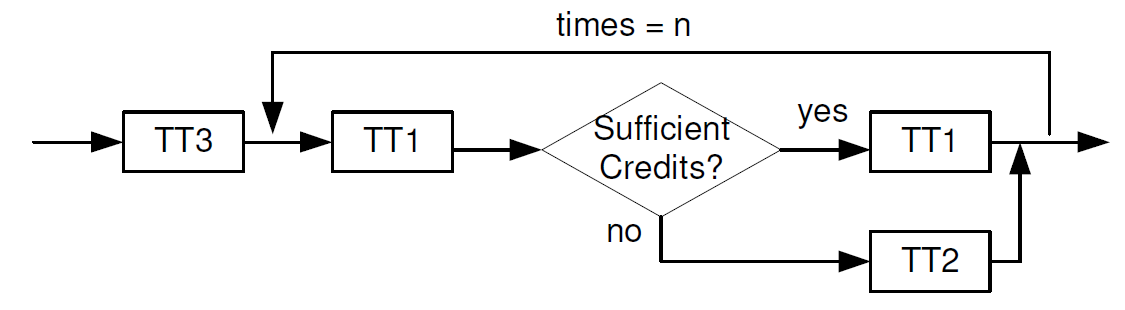
\includegraphics[scale=0.35]{img/Tsai2001ComplexTestScenario.png}
    \caption{Voorbeeld van een test case opgebouwd uit 3 verschillende thin-threads \autocite{Tsai2001}}
    \label{fig:tsaicomplexscenario}
\end{figure}

Om de test cases te vervolledigen tot reële gebruiksscenario's moet men ten slotte inputs kiezen op basis van de grenzen van de condities. Meestal gaat men \emph{grenswaarden} kiezen om te testen \autocite{Jorgensen2013}, maar dit kan ook door: de input \emph{willekeurig} te selecteren \autocite{Loo1988}, de mogelijke inputs in \emph{categorieën} te sorteren en daar representatieve data uit halen of door eenvoudigweg data uit de reële gebruiksomgeving te gebruiken (\emph{``usage-based testing''}) \autocite{Dyer1992}.

Thin threads steunen inherent op \textbf{reusability}, wat de opbouw van een test automatisatiesysteem niet alleen versnelt maar ook de kwaliteit en onderhoudbaarheid van het systeem ten goede komt \autocite{LombardHill2014}. De specifieke implementatie van thin threads is afhankelijk van het gebruikte framework. In de praktijk zullen dit vaak scripts zijn, hoewel elke vorm van hergebruik voordelig is \autocite{Madan2013} \autocite{Barrett2013}.

\subsubsection{Onderhoudbaarheid van een Test Automatisatiesysteem}

Het succes van een test automatisatieproject op de lange termijn is sterk afhankelijk van de onderhoudbaarheid van het systeem. Jim Holmes identificeert in zijn whitepaper ``Getting off on the Right Foot with Your Test Automation Project'' drie belangrijke problemen die de onderhoudbaarheid van web-based test automatisatiesystemen ondermijnen \autocite{Holmes2020}:

\begin{enumerate}
    \item Slecht gedefinieerde \textbf{``element locators''}.
    \item Synchronisatieproblemen bij \textbf{dynamische content}.
    \item Het niet consequent toepassen van \textbf{software engineering principes} zoals het \emph{Single Responsibility Principle} (SRP) en \emph{Don't Repeat Yourself} (DRY).
\end{enumerate}

De zogeheten ``locators'' laten toe dat het geautomatiseerde systeem elementen op een pagina kan vinden, bijvoorbeeld een input-element dat het syteem kan gebruiken om testdata in te voeren. Idealiter zijn deze locators:

\begin{itemize}
    \item \textbf{Flexibel}. Het gebruiken van het volledige pad van een element als locator is riskant; wijzigingen aan de structuur van pagina's maakt zulke locators snel onbruikbaar. Met unieke ID's, of tenminste vaste voor- en achtervoegsels voor bepaalde soorten elementen, kan men het gebruik van paden vermijden. Vaak is het ook mogelijk om elementen te selecteren op basis van één of meerdere criteria: types, klassen, inhoud, bovenliggende of onderliggende elementen, positie binnen een hiërarchie etc.
    \item \textbf{Gecentraliseerd}. Middels \emph{dictionaries} — die locators als sleutel/waarde-paren opslaan — of het \emph{page object pattern} — een recente techniek die pagina's als (objectgeoriënteerde) klassen met bijhorende attributen en methoden behandelt — kan men locators centraal beheren. Dit laat ook toe om locators te hergebruiken.
\end{itemize}

\begin{figure}[h!]
    \centering
    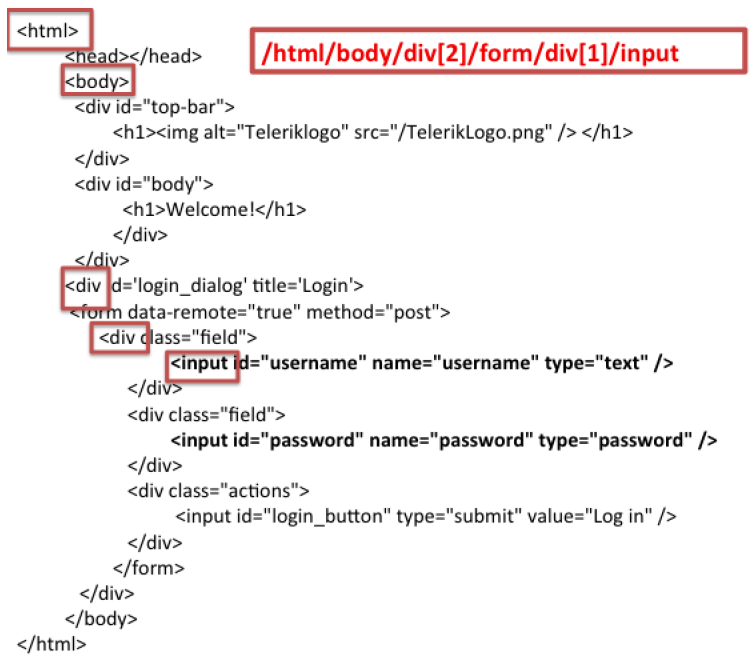
\includegraphics[scale=0.5]{img/Holmes2020XPath.PNG}
    \caption{Voorbeeld van een HTML-pagina met een input-element en de bijhorende locator op basis van het hiërarchische pad. \autocite{Holmes2020}}
    \label{fig:holmesxpath}
\end{figure}

De synchronisatieproblemen die optreden bij dynamische content worden vaak opgelost door expliciet te wachten tot aan bepaalde \emph{condities} voldaan wordt vooraleer verder te gaan naar de volgende stap. Een andere methode kan ontleend worden van Android Instrumentation testing: door gebruik te maken van het \emph{observer pattern} kan men wachten tot het gewenste resultaat beschikbaar is vooraleer verder te gaan met een test \autocite{Elye2018}. Dit vermijdt ook nodeloos wachten door gebruik te maken van een \emph{sleep}-functie.

Een andere belangrijke overweging is \textbf{test coverage} (testdekking): het aandeel van de code en de functionele vereisten zoals beschreven in de functionele specificatie dat in de (al dan niet geautomatiseerde) test cases gevalideerd wordt \autocite{Sheth2019}. Een dekkingsgraad van 100\% is niet in alle gevallen nodig om de kwaliteit van het opgeleverde softwareproduct te garanderen — sterker nog: eenmaal voorbij 90\% neemt de benodigde tijd om testen te implementeren voor het overblijvende deel sterk toe \autocite{Prause2017}.

\subsubsection{Beheer van Testdata}

Doorgaans worden testing frameworks ingedeeld in één van twee of drie groepen, op basis van hoe zij testdata beheren \autocite{Day2014} \autocite{Laukkanen2006}:

\begin{enumerate}
    \item \textbf{Data driven}. Dit type framework scheidt de testdata van de scripting logica door die eerste als sleutel-waarde paren op te slaan in een extern bestand (gaande van eenvoudige rekenbladen tot Open DataBase Connectivity). Testscenarios worden vaak met verschillende inputs (en corresponderende outputs) herhaald om alle mogelijk test cases af te dekken. Data driven frameworks leggen met andere woorden de nadruk op het verveelvuldigen van scenarios om de test coverage te vergroten.
    \begin{figure}[h!]
        \centering
        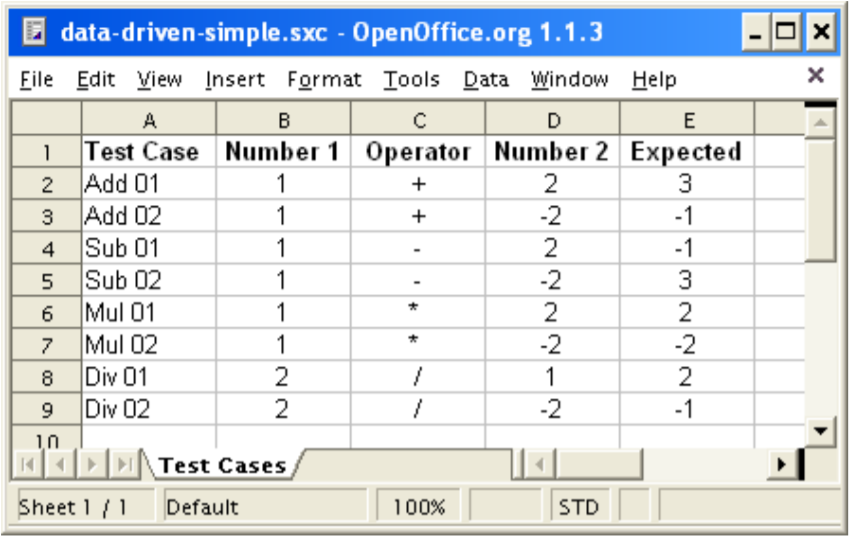
\includegraphics[scale=0.4]{img/Laukkanen2006DataDriven.PNG}
        \caption{Voorbeeld van sleutel-waarde paren die gebruikt worden binnen hetzelfde scenario, nl. de uitvoering van een binaire wiskundige operatie \autocite{Laukkanen2006}.}
        \label{fig:laukkanendatadriven}
    \end{figure}
    \item \textbf{Keyword driven}. Keyword driven frameworks focusen zich vooral op hergebruik en onderhoudbaarheid van de testen. Stukken code, geïdentificeerd a.d.h.v \emph{keywords}, worden geïsoleerd in externe bestanden (data tables) samen met eventuele data/locators. Testscenarios worden vervolgens samengesteld door keywords aan elkaar te rijgen. Dit zorgt ook voor een grotere mate van afhankelijkheid van het framework zelf \autocite{Madan2013}.
        \begin{figure}[h!]
        \centering
        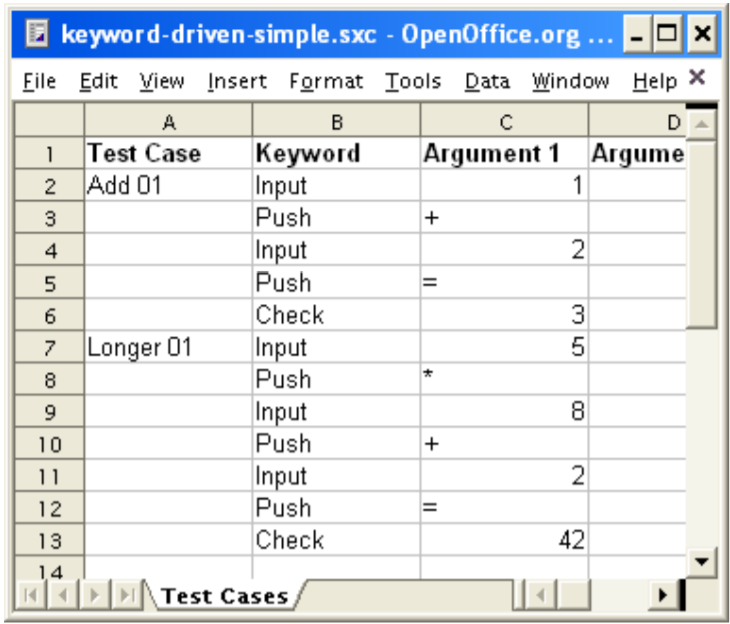
\includegraphics[scale=0.4]{img/Laukkanen2006KeywordDriven.PNG}
        \caption{Voorbeeld van test cases die opgebouwd worden uit keywords en bijhorende data \autocite{Laukkanen2006}.}
        \label{fig:laukkanenkeyworddriven}
    \end{figure}
    \item \textbf{Hybrid}. Hybride frameworks combineren bovenstaande technieken. De meeste mature frameworks lijken naar deze vorm te evolueren \autocite{Day2014}.
\end{enumerate}

\subsection{Overwegingen bij de Keuze voor een Test Automatisatiesysteem}

Test automatisatie vergt een substantiële initiële investering; analyse van de functionaliteit van de software, schrijven van testscripts, het introduceren van de tooling en het opleiden van personeel etc. \autocite{Kumar2016}. Het is dus van kritisch belang om een weloverwogen keuze te maken teneinde de kans op slagen van dergelijk project te maximaliseren. De volgende factoren zijn in het bijzonder belangrijk in acht te nemen:

\begin{itemize}
    \item \emph{De betrokken technologieën en omgevingen}. Het spreekt voor zich dat men voor het opzetten van test automatisatie anders te werk zal moeten gaan bij mainframe toepassingen dan voor webapplicaties. De beschikbare tooling zal ook afhankelijk zijn van de gebruikte technologieën (\cite{10.1145/1295014.1295062}).
    \item \emph{De beschikbare kennis}. Ervaring met een bepaald framework binnen het team is een sterke troef en vaak een doorslaggevende reden om een keuze te motiveren (\cite{Madan2013}).
    \item \emph{De lifecycle van de software}. Het te implementeren systeem dient te passen binnen het geplande levensverloop van de software zelf. Software waarvoor slechts een beperkt aantal toekomstige releases (of zelfs helemaal \emph{geen} toekomstige ontwikkeling) gepland is, zal niet gebaat zijn bij test automatisatie \autocite{Tiitinen2013}.
\end{itemize}

\section{e2e Testing Frameworks voor Angular}

\textbf{Angular}, het door Colruyt Group gekozen framework voor de nieuwe generatie van hun checkoutsysteem, is een open source framework voor het bouwen van Single Page Application (SPA)\footnote{Een \textbf{Single Page Application} zal op dynamische wijze één web pagina continu herschrijven met nieuwe data van de web server. Dit in tegenstelling tot de traditionele manier waar de browser bij de meeste handelingen van de gebruiker de volledige pagina herlaadt \autocite{Neoteric2016}.} ontwikkeld door Google. Het framework maakt voornamelijk gebruik van HTML en TypeScript (een uitbreiding van JavaScript). \autocite{AngularArchitecture}

De architectuur van Angular applicaties is gebaseerd op \textbf{NgModules} (``Angular modules'') die samenhorende componenten en services bevatten. Elke Angular app heeft minstens één NgModule: de \emph{root module} van waaruit de applicatie gelaunched wordt. Elk zichtbaar element (``view'') op Angular webpaginas wordt gestuurd door een \textbf{Component} dat de benodigde logica bevat en toegang heeft tot de relevante data. De view zelf wordt gerenderd aan de hand van een \textbf{template} die middels event en property binding met het component communiceert. Pagina's worden dan opgebouwd door Componenten te combineren en, waar nodig, te wisselen. \autocite{Tuzi2018,Garg2019,AngularArchitecture}

De correcte samenwerking tussen deze verschillende onderdelen wordt geverifiëerd door gebruikersinput te simuleren en de daaruit resulterende web pagina te valideren — i.e. E2E testing. Deze sectie gaat dieper in op de drie eerder genoemde kandidaat-frameworks voor het E2E testen van Angular applicaties.

\subsection{Protractor}

Protractor is een open source E2E testing framework voor AngularJS en Angular. Google, mede-ontwikkelaar van AngularJS en zijn opvolger Angular, bracht de eerste versie uit in 2013 \autocite{Amorim2014}.

Het framework bouwt verder op een aantal andere technologieën, zoals geïllustreerd wordt door onderstaand diagram. Een \textbf{web browser} dient als gebruikersinterface voor de Angular applicatie — enerzijds om web pagina's te renderen, en anderzijds om input te aanvaarden. In het geval van geautomatiseerde systemen heeft men een framework nodig om deze browser te automatiseren, hier is dat \textbf{Selenium} WebDriver. \textbf{WebDriver JS} is een javascript bindings implementatie voor Selenium die het test framework de benodigde APIs levert om testen geschreven in javascript  te kunnen uitvoeren. (\cite{TutorialspointProtractor2020})

\begin{figure}[h!]
    \centering
    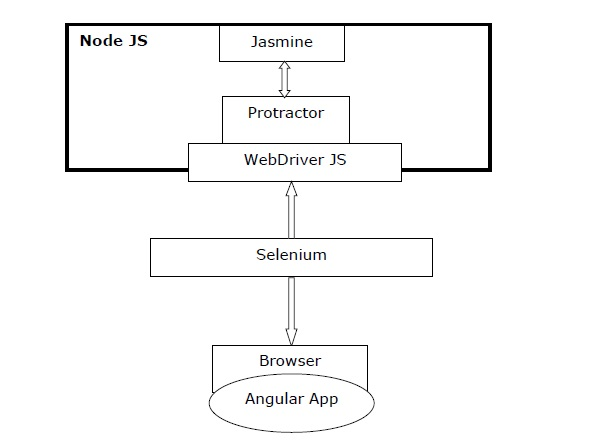
\includegraphics[scale=0.6]{img/TutorialsPointProtractor2020ProtractorDiagram.jpg}
    \caption{De structuur van een mogelijke stack die gebruik maakt van Protractor als end-to-end testing framework \autocite{TutorialspointProtractor2020}.}
    \label{fig:tutorialspointprotractordiagram}
\end{figure}

\textbf{Protractor} fungeert als een schil rond de Selenium WebDriver die toelaat gebruikersacties te simuleren (i.e. een \textbf{test runner}). Het framework biedt, naast een compactere syntaxis dan die beschikbaar in pure Selenium, ook een antwoord op de eerder besproken uitdagingen met name het beheren van locatoren en het omgaan met synchronisatieproblemen. (\cite{ToolsQA2019})

Protractor heeft ten slotte een \textbf{assertion framework} nodig om de testing interface te voorzien. De software tester schrijft zijn testen middels \textbf{assertions}: predicaten gebonden aan bepaalde punten in de software die toelaten te evalueren of de software onder gegeven voorwaarden de correcte toestand aanneemt \autocite{Alakeel2014}. Het assertion framework laat toe om die assertions op een compacte en gemakkelijk uitbreidbare manier uit toe voeren. Voor Protractor is \textbf{Jasmine} het standaard framework, maar dit kan ook een ander framework zijn. (\cite{SoftwareTestingHelp}).

Protractor biedt volgende relevante voordelen:
\begin{itemize}
    \item \textbf{Meerdere assertion libraries}. Standaard ondersteunt Protractor Jasmine, Mocha, Cucumber en Serenity/JS \autocite{ProtractortestFrameworks}.
    \item \textbf{Parallel testen over meerdere browsers}. De API van WebDriver JS is gebaseerd op \emph{promises}: elke functie heeft een promise als terugkeerwaarde, dewelke dient als plaatshouder voor het resultaat van een asynchrone functie. Dit, in combinatie met Selenium grid, laat toe om testen parallel te laten verlopen. (\cite{ProtractortestControlflow,Kamothi2019,TutorialspointProtractor2020}).
    \item \textbf{Auto-synchronisatie}. Protractor bouwt automatische wachtperioden in om het gebruik van expliciete \emph{waits} te vermijden — dit is vooral toepasselijk bij de locators specifiek aan Angular (o.a. \mintinline{TypeScript}{by.model()}, \mintinline{TypeScript}{by.binding()}, en \mintinline{TypeScript}{by.repeater()}) \autocite{Jarif2018}.
    \item \textbf{Cross-browser testing en headless browsers}. Protractor laat toe scripts in meerdere browsers uit te voeren, wat het mogelijk maakt op efficiënte manier de compatibiliteit van de applicatie met verschillende browsers te verifiëren. Het uitvoeren van tests op \emph{headless browsers} — i.e. browsers zonder grafische user interface — laat eveneens toe testen te versnellen doordat pagina's niet meer gerenderd moeten worden. \autocite{ToolsQA2019}
\end{itemize}

%Opm.: breaklines werkt enkel deftig als ik een spatie zet tussen by en het punt
Onderstaand voorbeeld illustreert het gebruik van het Page Object Model (POM, zie \cite{Mohsin2018}) alsook de Angular-specifieke locators (\mintinline[breaklines]{TypeScript}{by.model('yourName')} en \mintinline[breaklines]{TypeScript}{by .binding('yourName')}) in Protractor \autocite{ProtractortestPageobjects}. Het Page Object met bijhorende attributen en methoden wordt eerst gedefinieerd:

\begin{minted}[
    linenos,
    breaklines
]
{TypeScript}
var AngularHomepage = function() {
    var nameInput = element(by.model('yourName'));
    var greeting = element(by.binding('yourName'));

    this.get = async function() {
        await browser.get('http://www.angularjs.org');
    };

    this.setName = async function(name) {
        await nameInput.sendKeys(name);
    };

    this.getGreetingText = function() {
        return greeting.getText();
    };

    // Not async, returns the element
    this.getGreeting = function() {
        return greeting;
    };
};
module.exports = new AngularHomepage();
\end{minted}

Dit Page Object kan dan gebruikt worden in de uitvoering van (asynchrone) testen:

\begin{minted}[
    linenos,
    breaklines
]
{TypeScript}
var angularHomepage = require('./AngularHomepage');
describe('angularjs homepage', function() {
    it('should greet the named user', async function() {
        await angularHomepage.get();

        await angularHomepage.setName('Julie');

        expect(await angularHomepage.getGreetingText()).toEqual('Hello Julie!');
    });
});
\end{minted}

\subsection{Cypress}

Cypress, eveneens een open source E2E testing framework, werd in 2018 gereleased door een onafhankelijk team geleid door Brian Mann \autocite{Mann2017,Mann2018}.

In tegenstelling tot de meeste E2E testing frameworks, die buiten de browser runnen en opdrachten over het netwerk heen uitvoeren, is Cypress geïntegreerd in dezelfde run loop als de applicatie die getest wordt \autocite{Bharadwaj2018,Cypress1}. Figuur ~\ref{fig:vierbergencypressarchitecture} illustreert de werking van het framework. Het browser window bevat zowel de applicatie als Cypress in hun eigen iFrames. Middels een proxy communiceert de browser met een Nodejs-proces dat fungeert als substituut voor de backend. Omdat de gebruikte proxy deel is van Cypress is het mogelijk om requests en responses te onderscheppen en waar nodig te wijzigen of mocken \autocite{Vierbergen2019}.

\begin{figure}[h!]
    \centering
    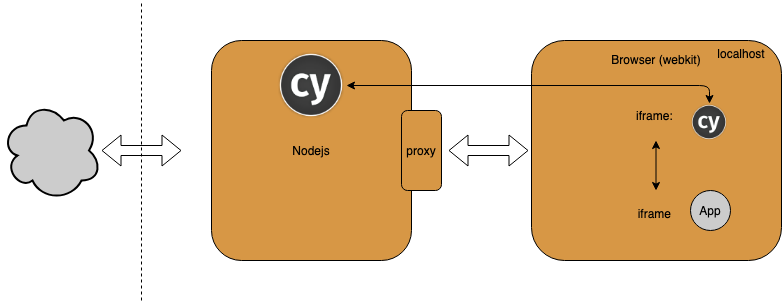
\includegraphics[scale=0.4]{img/Vierbergen2019CypressArchitecture.png}
    \caption{Architectuur van het Cypress testing framework \autocite{Vierbergen2019}.}
    \label{fig:vierbergencypressarchitecture}
\end{figure}

Deze structuur geeft Cypress de volgende voordelen:
\begin{itemize}
    \item \textbf{Snelheid}. Cypress runt rechtstreeks in de browser en is daardoor veel sneller dan frameworks die remote werken, zoals die Selinium gebruiken.
    \item \textbf{Controle}. De tester heeft rechtstreekse toegang tot netwerkverkeer en host objecten, wat hem meer controle geeft (o.a. directe DOM manipulatie) en toelaat de applicatie gemakkelijker te debuggen.
    \item \textbf{Automatisch wachten}. Cypress wacht automatisch tot de volledige pagina geladen werd en alle asynchrone requests afgehandeld werden vooraleer te beginnen met een test.
    \item \textbf{Real-time reloading}. By het opslaan van testbestanden zal Cypress de test automatisch opnieuw runnen.
    \item \textbf{Alles-in-één}. Het is niet nodig om meerdere tools te installeren en te laten samenwerken zoals bij vele andere frameworks wél het geval is.
    \item \textbf{Ondersteunt alle JavaScript frameworks}. Elk op JavaScript gebaseerd framework — waaronder Angular, React, Vue en Elm — kan gebruik maken van de mogelijkheden die Cypress biedt \autocite{Karen2019}.
    \item \textbf{Headless browsers}. Ook Cypress kan headless gerund worden \autocite{Karen2019}.
\end{itemize}

Er zijn echter ook een aantal belangrijke nadelen. Ten eerste is Cypress gespecialiseerd in end-to-end testing — elk andere soort testing, bijvoorbeeld unit testing, vereist een bijkomstige tool of pakket \autocite{McPeak2018}. Ten tweede ondersteunt Cypress enkel Chrome als browser voor het runnen van testen \autocite{Leners2020}. Dit zorgt ervoor dat opgebouwde expertise in het gebruik van Cypress minder overdraagbaar is dan E2E testing frameworks die meer technologieën ondersteunen.

Mocha en Chai worden hoofzakelijk gebruikt om Cypress testen te schrijven, hoewel er ook integraties zijn met andere technologieën zoals Cucumber \autocite{Jordi2019}.

Een voorbeeld van een test geschreven in Cypress wordt hier onder gegeven \autocite{Vierbergen2019}. Merk op dat de functies \mintinline[breaklines]{JavaScript}{context()} en \mintinline[breaklines]{JavaScript}{it()} — die ontleend werden aan Mocha — vervangen kunnen worden door respectievelijk \mintinline[breaklines]{JavaScript}{describe()} en \mintinline[breaklines]{JavaScript}{specify()} \autocite{Cypress2}.

\begin{minted}[
    linenos,
    breaklines
]
{JavaScript}
context('Clients test', () => {
    beforeEach(() => {
        cy.visit('/clients')
    })
    
    it('Clients page should have Clients as a title', () => {
        cy.get('.table-container-header h1').contains('Clients');
    });
    
    it('Clients table should initially have 20 rows', () => {
        cy.get('.mat-row').then(($rows) => {
            expect($rows.length).to.be.eq(20);
        });
    });
    
    it('Clients table should show 10 rows when pagesize is set to 10', () => {
        cy.get('mat-select').click();
        cy.get('mat-option').contains('10').then(option => {
            cy.wrap(option).contains('10');
            option[0].click();
            cy.get('mat-select').contains('10');
            cy.get('.mat-row').then(($rows) => {
                expect($rows.length).to.be.eq(10);
            });
        });
        
    });
})
\end{minted}

Elementen worden in cypress geselecteerd middels \mintinline[breaklines]{JavaScript}{cy.get()} die elk type selector of een alias kan bevatten. Interactie met het geselecteerde element wordt vervolgens verwezenlijkt met commando's zoals \mintinline[breaklines]{JavaScript}{.click()}, \mintinline[breaklines]{JavaScript}{.type()} en \mintinline[breaklines]{JavaScript}{.check()}. Commando's zoals \mintinline[breaklines]{JavaScript}{.contains()}, \mintinline[breaklines]{JavaScript}{.find()} en \mintinline[breaklines]{JavaScript}{.should()} kunnen waar nodig aan \mintinline[breaklines]{JavaScript}{cy.get()} geregen worden om het resultaat te verfijnen. Het gebruik van HTML \mintinline[breaklines]{HTML}{data-*} attributen wordt door het Cypress team aangemoedigd als best practice voor locators. \autocite{CypressGet,CypressInteractingWithElements,CypressBestPractices}

Zoals vermeld is het mogelijk om backend calls te onderscheppen en mockdata terug te sturen. Dit is mogelijk door een server te runnen met \mintinline[breaklines]{JavaScript}{cy.server()} en de te onderscheppen routes en de terug te sturen mockdata te definiëren \autocite{Vierbergen2019}:

\begin{minted}[
linenos,
breaklines
]
{JavaScript}
beforeEach(() => {
    cy.server();
    cy.route('GET', '**/*/api/client-service/**/*',
    {
        "content":[
        {
            "id":18,
            "firstName":"Tatiana",
            "lastName":"Velez",
            "email":"diam.dictum@Proin.net",
            "birthday":"626286135",
            "city":"Dumfries",
            "zip":"694245"
        }
        ],
        "pageable":{
            "sort": {
                "sorted":true,
                "unsorted":false
            },
            "pageSize":20,
            "pageNumber":0,
            "offset":0,
            "paged":true,
            "unpaged":false
        },
        "last":false,
        "totalElements":1,
        "totalPages":1,
        "first":true,
        "sort":{
            "sorted":true,
            "unsorted":false
        },
        "numberOfElements":1,
        "size":1,
        "number":0
    }
    ).as('stub-clients');   
    cy.visit('/clients');
})
\end{minted}

Ten slotte biedt Cypress twee mogelijkheden om testen de debuggen. Enerzijds zijn er ``Snapshots'': bepaalde waarden worden uitgeschreven in snapshotbestanden zodat de ontwikkelaar deze na de test kan controleren en kan gebruiken als verwachte waarden in herhalingen van de test. Anderzijds laten de commando's \mintinline[breaklines]{JavaScript}{cy.pause()} en \mintinline[breaklines]{JavaScript}{cy.debug()} toe om respectievelijk de uitvoering van een test te pauzeren en om extra logging te bekomen in de console van de browser. \autocite{CypressSnapshot2018,Noring}

\subsection{UFT}

Unified Functional Testing (UFT) is een softwarepakket dat HP's QuickTest Professional (QTP) en Service Test verenigt. De software werd in 2001 voor het eerst gereleased werd en wordt sinds 2016 door Micro Focus onderhouden \autocite{Swati2020,LearnQtpWhatIs}.

UFT verschilt op een aantal belangrijke punten met Protractor en Cypress:
\begin{itemize}
    \item Eerst en vooral is het een beduidend ouder pakket; wat vandaag gekend is als ``UFT'' werd voor het eerst in \textbf{2001} beschikbaar gemaakt, terwijl Protractor en Cypress pas in 2013 en 2018 (respectievelijk) uitgebracht werden \autocite{Swati2020,Mann2018,Amorim2014}.
    
    \item Ten tweede is de software gecommercialiseerd en enkel beschikbaar bij aanschaf van een \textbf{licentie}, terwijl Protractor en Cypress open source zijn \autocite{Guru99SeleniumUFTDifference,VSoftUFTvsSelenium,Mann2017,Kumar}.

    \item Ten derde zijn Protractor en Cypress gespecialiseerd in web applicaties, terwijl UFT alle soorten \textbf{client-server applicaties} kan testen — dus ook desktop applicaties \autocite{Tribbiani2017,Cypress1,Amorim2014}.

    \item Ten vierde biedt UFT twee interfaces voor het schrijven van tests. De eerste is de \textbf{``expert view''} die de gebruiker de broncode — UFT gebruikt VBScript als scripting taal \autocite{Rajkumar2017} — van een test laat editeren. De tweede is de \textbf{``keyword view''}: een grafische user interface die het niet-technische testers mogelijk maakt testen te schrijven \autocite{Guru99WhatIsQTPUFT}.
\end{itemize}
UTF testen bestaan uit \emph{``acties''}, die kunnen worden hergebruikt wat modulariteit promoot. Zulke acties zijn elementaire handelingen zoals 'log in', 'schrijf en stuur email' en 'log uit'. Een test is met andere woorden een opeenvolging van verschillende acties die uitgevoerd worden, met verschillende parameters voor individuele testen.
%%%%%%%%%%%%%%%%%%%%%%% REFERENTIE NODIG %%%%%%%%%%%%%%%%%%%%%%%%%%%

Onderstaande figuur illustreert de opbouw van een UFT actie — in dit geval 'log in' — gebruik makende van de keyword view. Elk stap van de actie is een operatie die uitgevoerd wordt op een item: een object, een VBScript statement of een function call kan zijn. Deze operatie krijgt doorgaans een ``waarde'' (parameters of argumenten) en kan eventueel aangevuld worden met commentaar (``documentatie''). Merk het gebruik van een \textbf{objecthiërarchie} op: het item 'login' is een dialoog die de gebruiker vraagt 2 velden in te vullen, met name 'Agent Name' en 'Password'. \autocite{SwatiWorkingWithKeywordView2020}

\begin{figure}[h!]
    \centering
    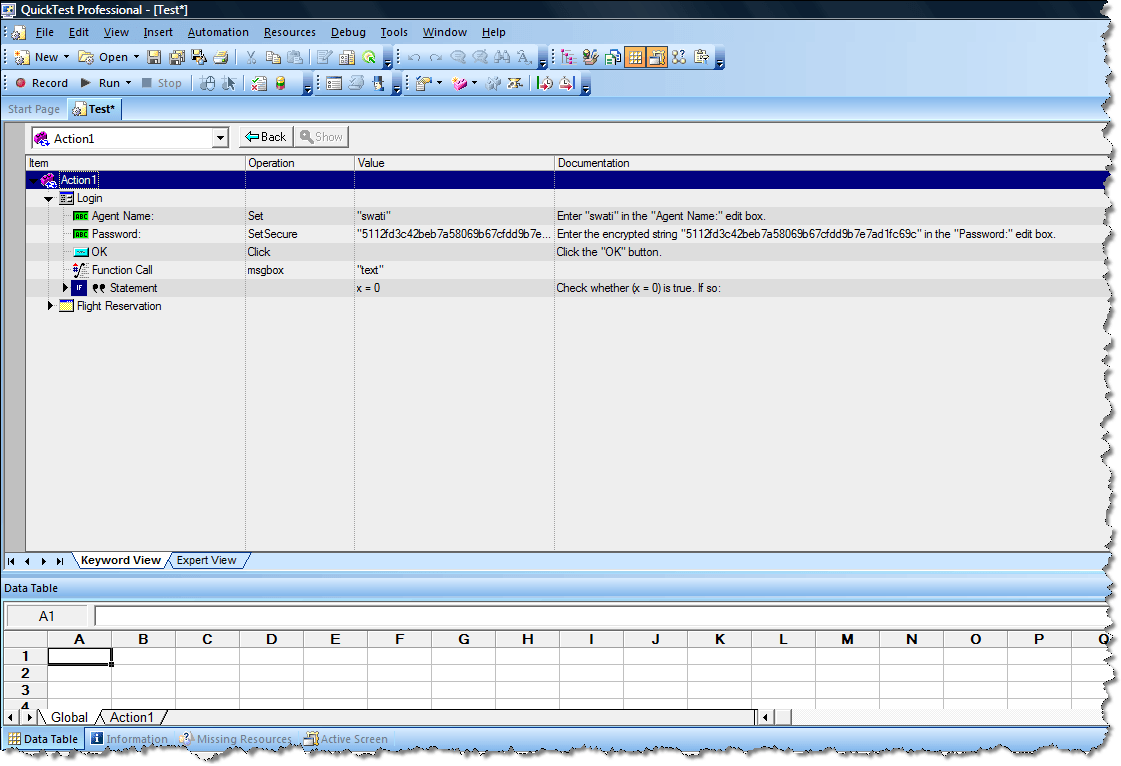
\includegraphics[scale=0.5]{img/Swati-QTPKeywordScreen.png}
    \caption{User interface van de keyword view in QTP \autocite{SwatiWorkingWithKeywordView2020}.}
    \label{fig:utfkeywordview}
\end{figure}

Deze actie kan in de expert view als volgt geschreven worden \autocite{SwatiWorkingWithKeywordView2020}:

\begin{minted}[
linenos,
breaklines
]
{VBScript}
    Dialog("Login").WinEdit("Agent Name:").Set "swati"
    Dialog("Login").WinEdit("Password:").SetSecure "5112fd3c42beb7a58069b67cfdd9b7e7ad1fc69c"
    Dialog("Login").WinButton("OK").Click
    msgbox "text"
    If x=0 Then
    msgbox "text 2"
    End If
    Window("Flight Reservation").ActiveX("MaskEdBox").Type "010312"
    Window("Flight Reservation").WinComboBox("Fly From:").Select "Denver"
    Window("Flight Reservation").WinComboBox("Fly To:").Select "Frankfurt"
\end{minted}

% Zie object model -- https://admhelp.microfocus.com/uft/en/all/AutomationObjectModel/Default.htm

%data-driven testing


%


\subsection{Behavior Driven Development Frameworks}

\lipsum[9]

\subsubsection{Mocha}

\lipsum[8-9]

\subsubsection{Jasmine \& Karma}

\lipsum[8-9]

\subsubsection{Cucumber}

\lipsum[8-9]